\graphicspath{{./fourth/img/}} % path to graphics

\section*{\LARGE Введение}
\addcontentsline{toc}{section}{Введение}
Дискретно-событийное моделирование зародилось примерно тогда же, когда
появилась системная динамика. В 1961 году инженер компании IBM Джеффри
Гордон представил программу GPSS, которая считается первой реализацией
метода моделирования на основе дискретных событий. В наши дни существует
множество различных программных инструментов для дискретно-событийного
моделирования, в том числе и современная версия GPSS.\par
Модель задается графически в виде диаграммы процесса, блоки которой
представляют собой отдельные операции. Как правило, диаграмма процесса
начинается с блока «источник», генерирующего агентов. Этот блок передает
агентов в последующие блоки диаграммы, задающие операции моделируемого
процесса. Завершается диаграмма процесса обычно блоком, уничтожающим
этих агентов.\par
Мы промоделируем производственные процессы в небольшом заводском цеху:

\begin{itemize}
	\item Каждый час на завод приезжает грузовик с поддонами. На каждом
		поддоне находится заготовка, готовая к обработке в данном цеху.
	\item Все находящиеся на грузовике поддоны разгружаются
		в приемной зоне цеха.
	\item  Далее эти поддоны с помощью автопогрузчиков помещаются в
		подготовительную зону хранения.
	\item По прошествии определенного времени поддоны с заготовками
		доставляются автопогрузчиками к станку с ЧПУ. Здесь происходит
		обработка заготовок --- производство конечных изделий.
\end{itemize}

\clearpage

\section*{\LARGE Выполнение практической работы}
\addcontentsline{toc}{section}{Выполнение практической работы}

\section{Создание простой модели}
Мы начнем с создания простой модели, имитирующей появление поддонов в
приемной зоне заводского цеха и их последующее пребывание в зоне хранения.\par
AnyLogic добавляет изображение на диаграмму Main в его исходном размере, но
вы можете изменить длину или ширину изображения. Если вы исказили
пропорции изображения (как это показано на следующем рисунке), то вы
можете восстановить исходные размеры изображения, щелкнув по кнопке
\textbf{Восстановить исходный размер} на странице свойств
этого изображения.\par
Нашим следующим шагом будет рисование элементов из палитры \textbf{Разметка
пространства} поверх плана фабричного цеха. Мы создадим транспортную сеть с
помощью путей и узлов.\par
Далее нарисуем сеть, задающую пути перемещения поддонов в нашей
модели. Вначале нарисуйте прямоугольный узел у входа в цех. Этот узел будет
представлять в нашей модели приемную зону для поддонов.
Затем давайте нарисуем путь перемещения автопогрузчиков в нашей модели
и пути, которые соединят оба нарисованных
ранее узла с сетью склада. Вначале нарисуем путь, соединяющий сеть
склада с узлом у входа в цех (\texttt{receivingDock}). Следом
давайте создадим диаграмму моделируемого нами процесса из блоков
библиотеки.\par
Теперь можем добавить логику
управления складом, и для того мы воспользуемся блоками \textbf{Библиотеки
производственных систем}. Блок Store моделирует помещение поддонов
в заданные ячейки склада.
Как вы заметили, мы соединяем правый порт одного блока с левым портом
следующего блока. У каждого блока имеется левый входной порт и правый
выходной порт, и вы можете соединять входные порты только с выходными.\par

На данном этапе, создана простейшая дискретно-событийной модели, и теперь можно
запустить ее и понаблюдать за поведением агентов
(Рисунок~\ref{fig:model:easy}).

\begin{image}
	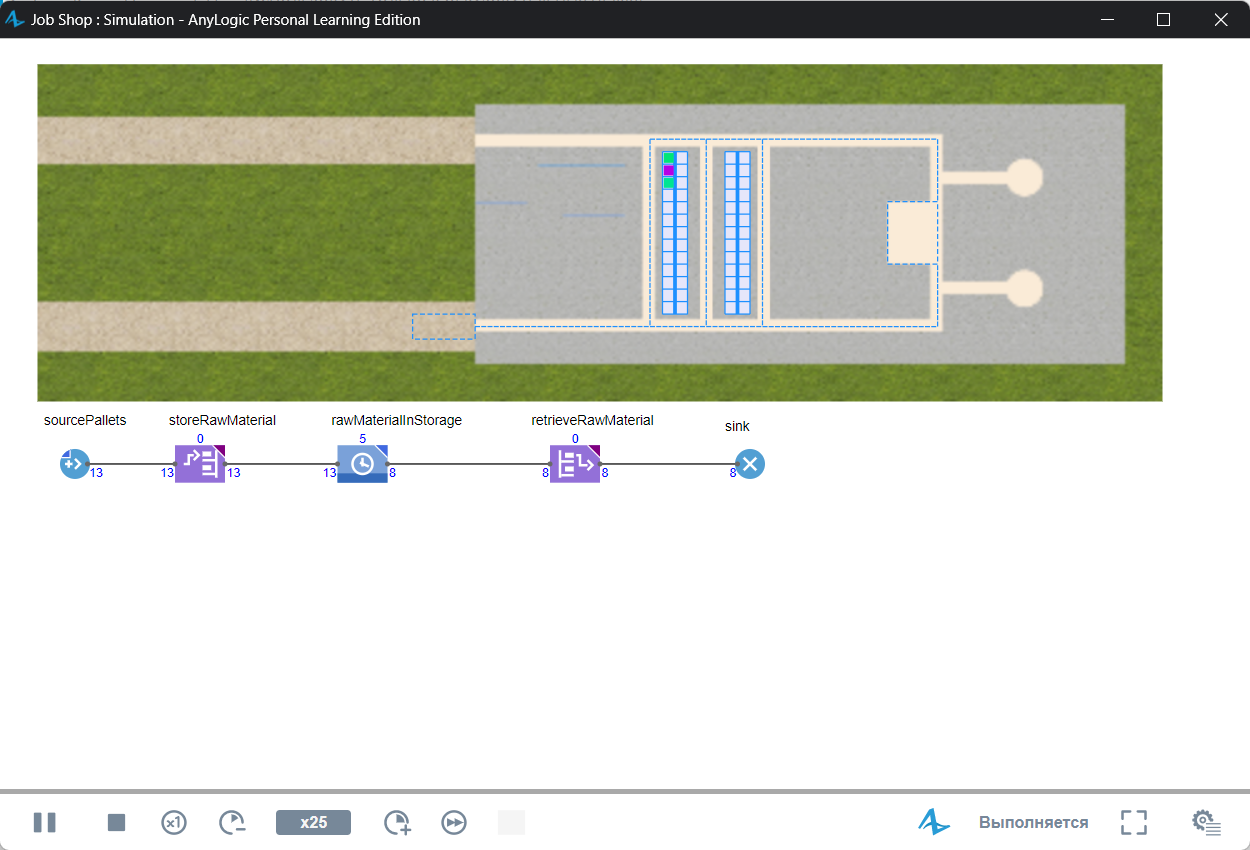
\includegraphics[width=0.9\textwidth]{2023-04-02_14-52-52}
	\caption{Простейшая дискретно-событийной модель}
	\label{fig:model:easy}
\end{image}

\section{Добавление ресурсов}
Продолжим создание нашей модели. Теперь мы добавим ресурсы
(автопогрузчики), с помощью которых будет производиться как помещение
поддонов в стеллаж, так и их последующее перемещение в производственную
зону.\par
Ресурсами называются объекты, используемые агентами для выполнения
определенной операции. В случае необходимости агент должен получить
ресурс, выполнить операцию, а затем освободить ресурс.\par
Ресурсами нашей модели являются автопогрузчики, перемещающие поддоны из
зоны разгрузки в стеллаж, а затем доставляющие поддоны из стеллажа в
производственную зону.
Каждый набор ресурсов задается в AnyLogic блоком библиотеки
\textbf{ResourcePool}.\par
Задав ресурсы, теперь нужно сделать так, чтобы блоки диаграммы
процесса нашей модели использовали эти ресурсы.\par
При перемещении агента блок \texttt{Store} захватывает свободный ресурс
(автопогрузчик), перемещает его в место расположения агента (поддона),
прикрепляет ресурс к агенту, перемещает агента с помощью ресурса в ячейку
склада, а затем освобождает ресурс. Схожим образом ведет себя и блок
\texttt{Retrieve} (разница в том, что он извлекает поддоны со склада).\par
Запустив модель, вы увидите, как автопогрузчики забирают поддоны из зоны
разгрузки и помещают их на склад. По истечении небольшой задержки они
перемещают поддоны в зону парковки автопогрузчиков, при попадании
в которую поддоны исчезают (Рисунок~\ref{fig:model:res}).

\begin{image}
	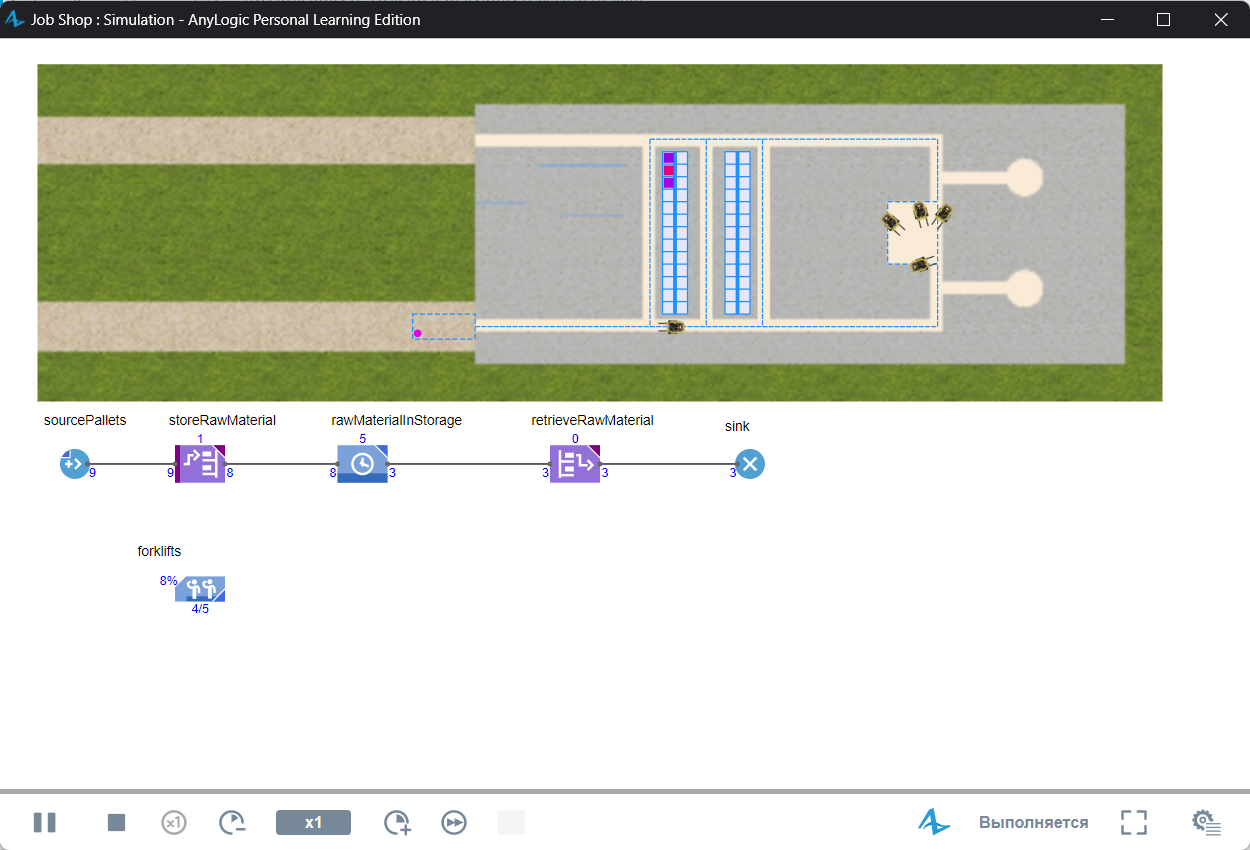
\includegraphics[width=0.9\textwidth]{2023-04-02_14-57-12}
	\caption{Использование ресурсов в модели}
	\label{fig:model:res}
\end{image}

\section{Создание трехмерной анимации}
Давайте теперь добавим трехмерную анимацию моделируемого нами процесса.
Начнем с добавления камеры.\par
Камера "снимает" ту сцену, которую вы видите в окне трехмерной анимации.
Добавив в вашу модель камеру, вы можете выбрать, что именно вы хотите
видеть в 3D окне.\par
В этом разделе мы использовали стены исключительно для анимационных
целей. На самом деле стены чаще используются в пешеходном
моделировании для задания стен и других препятствий для движения
людей.\par
AnyLogic создаст тип агента \textbf{Pallet} и откроет в редакторе графическую
диаграмму этого типа. В левом верхнем углу холста (а именно, в точке
начала координат) вы увидите фигуру анимации, выбранную нами только что
в мастере создания типа агента.\par
Нашим следующим шагом будет добавление фигуры коробки поверх фигуры
анимации поддона. Поскольку мы будем работать с объектами небольшого
размера, сначала давайте увеличим масштаб диаграммы.\par
Если вы откроете свойства блока \textbf{sourcePallets}, то вы увидите,
что в свойстве Новый агент выбран тип \textbf{Pallet}. Это значит,
что данный блок будет создавать агентов типа \textbf{Pallet} .\par
Запустив модель увидем, что поддоны отображаются натуралистичными трехмерными
моделями. Однако если вы увеличите масштаб трехмерного изображения, то вы
заметите, что поддоны расположены чуть в стороне от вил погрузчиков
(Рисунок~\ref{fig:model:camera}).

\begin{image}
	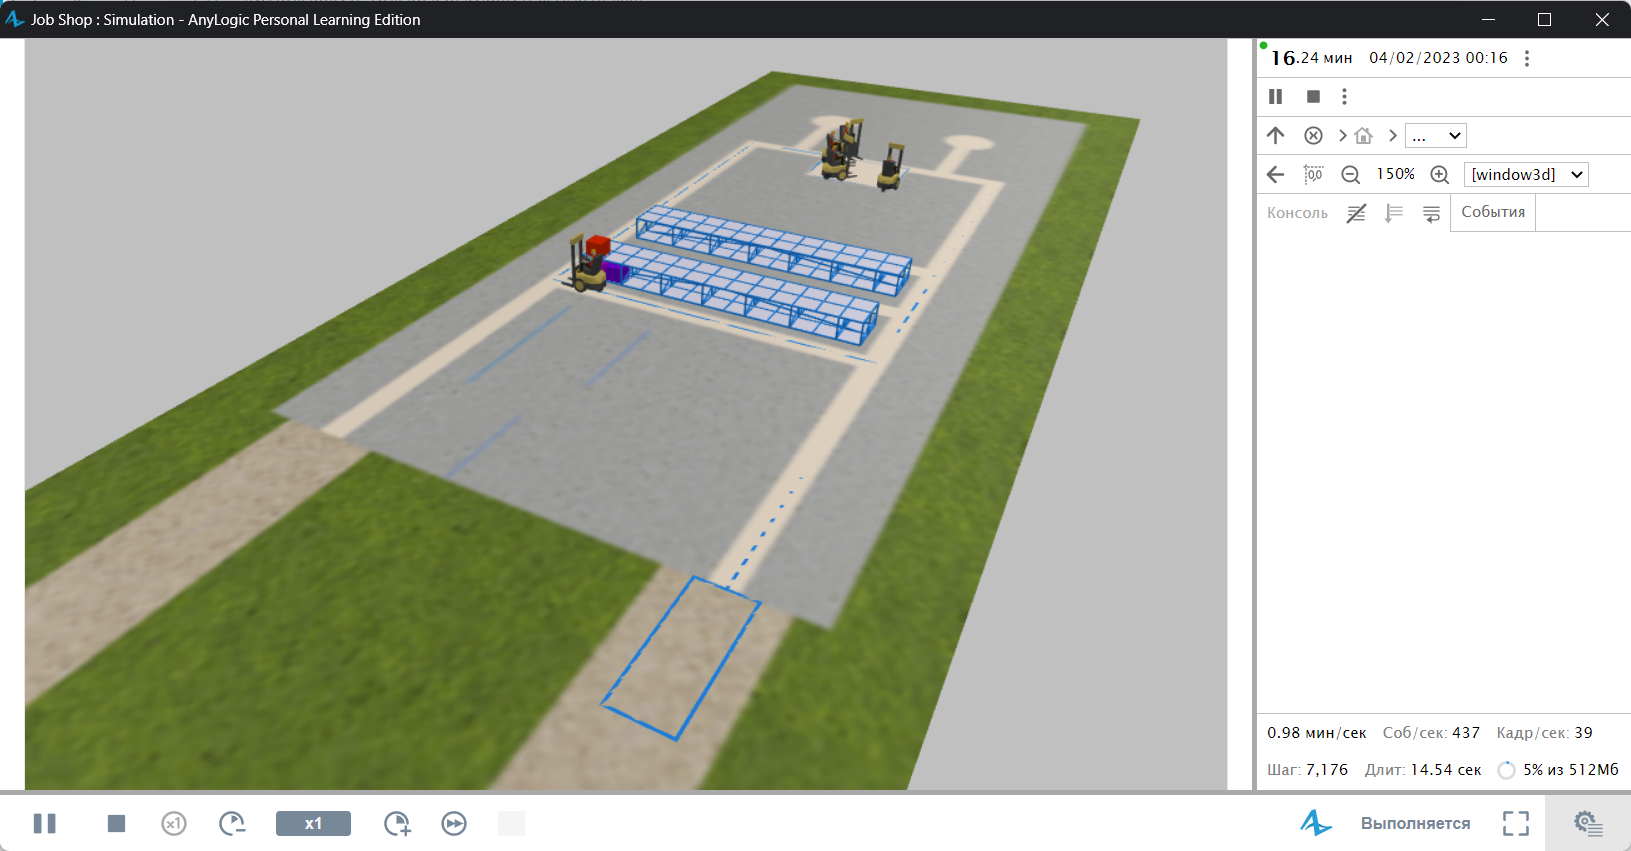
\includegraphics[width=0.9\textwidth]{2023-04-02_15-11-00}
	\caption{Использование камеры в модели}
	\label{fig:model:camera}
\end{image}

Давайте устраним эту неточность.\par
В то же время, во время нахождения на стеллажах поддоны с коробками
отображаются не трехмерными моделями, а кубиками разных цветов. Это
сделано специально для повышения производительности модели, но при
желании эту настройку можно отключить.\par
Запустите модель и увидите, что теперь объекты визуализируются
трехмерными моделями и находясь на стеллаже склада
(Рисунок~\ref{fig:model:padd}).

\begin{image}
	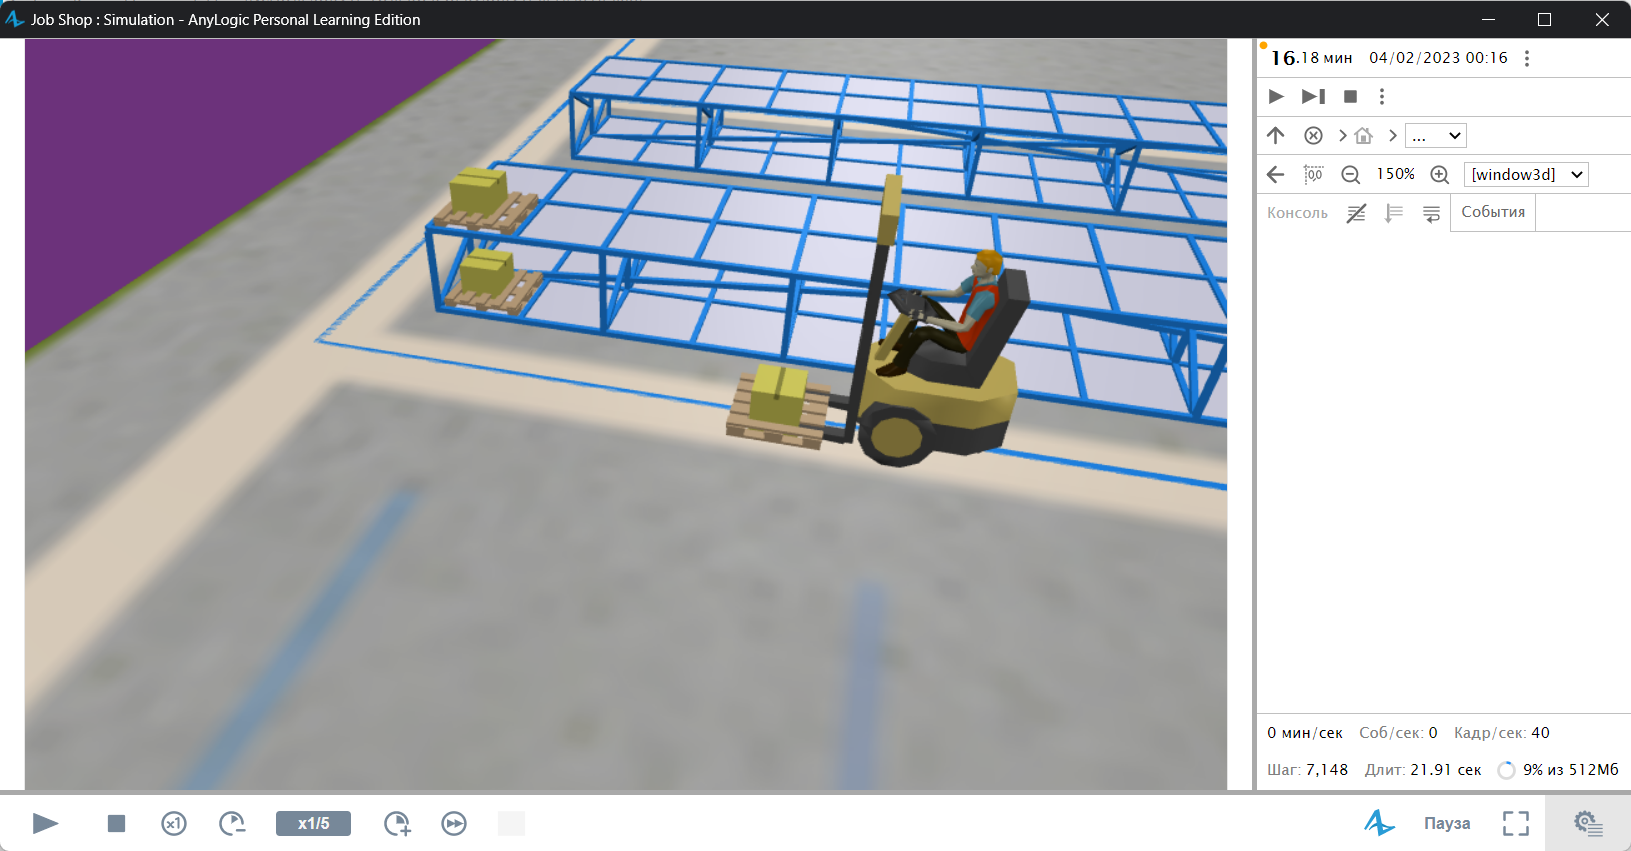
\includegraphics[width=0.9\textwidth]{2023-04-02_15-28-11}
	\caption{Использование трехмерных объектов}
	\label{fig:model:padd}
\end{image}

\section{Моделирование доставки поддонов фурами}
На этом этапе обучения мы добавим фуры, доставляющие поддоны на завод.
Начнем с создания еще одного типа агента, задающего фуру.\par
Добавим в нашу сеть два новых элемента: узел, в котором будут появляться
фуры, и путь, по которому они будут следовать до приемной зоны.\par
Продолжительность операции определяется скоростью разгрузки и отвоза
поддонов автопогрузчиками. Мы будем считать эту операцию выполненной,
когда блок \textbf{Store} завершит установку поддонов на хранение,
и смоделируем это изменением режима работы блока \textbf{Delay}.\par
Как правило вы будете задавать Время задержки для работы блока \textbf{Delay}.
Время может быть фиксированным, например, равным пяти минутам, или быть
стохастическим (случайным), т.е. определяться функцией распределения
вероятности, например: \texttt{triangular(1, 2, 6)}.\par
Два блока \textbf{Source} нашей модели создают агентов двух разных типов:
фуры, появляющиеся каждый час, и поддоны, появляющиеся каждые пять минут.
Поскольку нам нужно, чтобы поддоны появлялись при разгрузке фуры, мы
изменим настройки того блока \textbf{Source}, который генерирует поддоны.\par
Давайте сделаем так, чтобы первая фура появлялась при запуске модели, и нам
не нужно было ждать ее появления целый час модельного времени.\par
Когда требующие разгрузки поддоны заканчиваются, операция блока unloading
завершается (путем вызова его функции \texttt{stopDelayForAll()}).
При этом фура покидает блок unloading и поступает в следующий блок
диаграммы процесса: \texttt{drivingToExit} .\par
Аттракторы можно добавить, перетаскивая их по отдельности из палитры, но
если они образуют регулярную структуру, то проще будет добавить их всех
разом с помощью специального мастера. У этого мастера имеется несколько
режимов создания, он также способен удалить все аттракторы узла. Открыть
мастер можно, щелкнув по кнопке \texttt{Aттракторы...}
в панели свойств узла.\par
Теперь анимация процесса разгрузки фуры должна будет выглядеть
как показано на рисунке~\ref{fig:model:truck}.

\begin{image}
	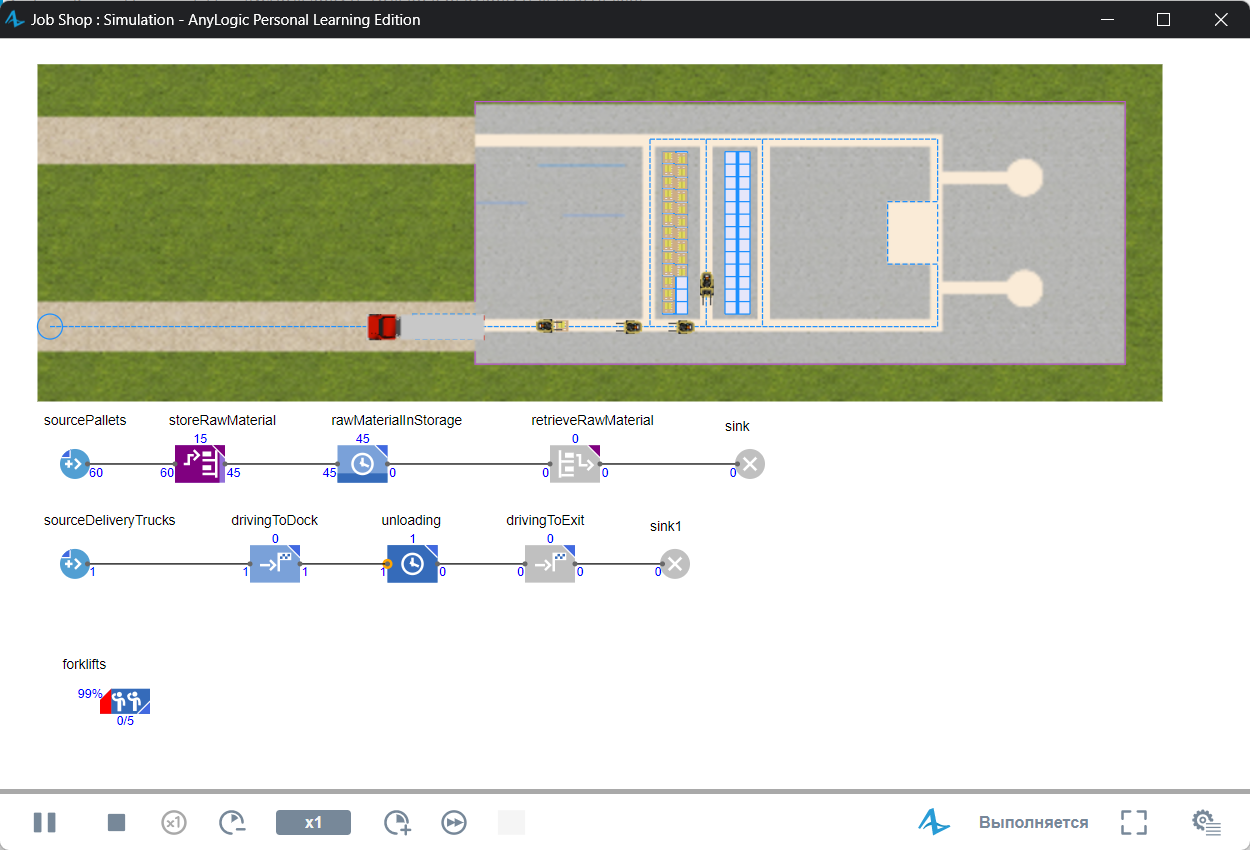
\includegraphics[width=0.9\textwidth]{2023-04-02_15-46-36}
	\caption{Добавление фуры в модель}
	\label{fig:model:truck}
\end{image}

\section{Моделирование станков с ЧПУ}
На этом этапе обучения мы добавим в модель станки с ЧПУ, на которых будет
производиться изготовление готовой продукции.\par
Давайте начнем с задания мест расположения станков с помощью точечных
узлов. Нам потребуется нарисовать пути, чтобы подключить оба эти узла к нашей
сети. Эти пути потребуются автопогрузчикам для подъезда к станкам.\par
В нашем случае станок с ЧПУ --- это ресурс, поэтому мы добавим его в нашу
модель, создав новый тип ресурса с помощью блока \textbf{ResourcePool}.\par
Завершив задание набора ресурсов, нам нужно создать новый его тип.\par
Теперь мы готовы изменить диаграмму процесса, описывающую поведение
поддонов: мы добавим блок \textbf{Seize}, который будет занимать
ресурс-станок. Следующий за ним блок Delay будет моделировать обработку
заготовок на станке, а блок Release будет освобождать станок с ЧПУ,
делая его готовым для обработки заготовок со следующего поддона.\par
Как вы помните, в диаграмме процесса уже есть блок
\texttt{retrieveRawMaterial},
моделирующий доставку поддонов в зону парковки автопогрузчиков.\par
Когда вы запустите модель, то увидите, что хотя процессы и смоделированы
верно, но на трехмерной анимации поддоны отображаются прямо по центру
фигуры анимации станка с ЧПУ. Это происходит потому, что и станок, и
обрабатываемый им поддон используют один и тот же точечный узел для
отображения анимации. Чтобы решить эту проблему, нам необходимо
переместить станок с ЧПУ вправо и повернуть его так, чтобы он был обращен к
поддону.\par
Давайте используем для анимации станка два схожих объекта трехмерной
анимации, один из которых будет представлять станок в режиме ожидания, а
второй --- в процессе обработки заготовок. У этих объектов мы настроим
значения свойства Видимость, благодаря чему наша модель будет отображать
ту или иную фигуру в зависимости от текущего состояния станка.\par
Когда вы задаете выражение для динамического значения свойства, по ходу
выполнения модель будет вычислять это выражение на каждом кадре анимации
и применять вычисленное значение в качестве текущего значения свойства. С
помощью этой возможности пользователи AnyLogic могут анимировать свои
модели, задавая динамические значения для координат, размерностей или
цвета графических объектов.\par
Итоговая диаграмма показана на рисунке~\ref{fig:model}.

\begin{image}
	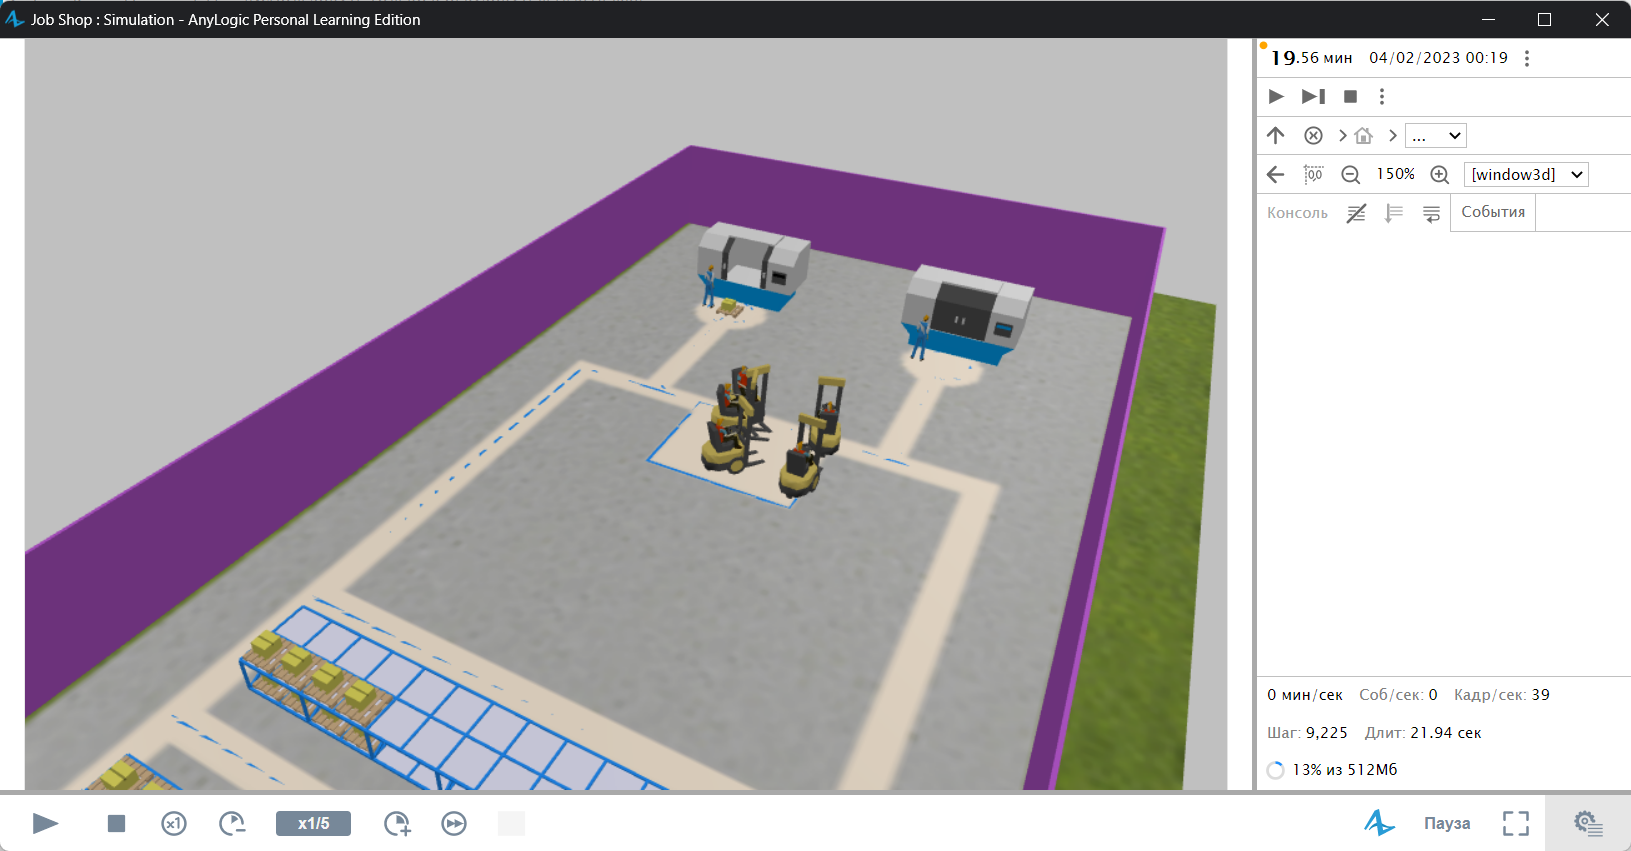
\includegraphics[width=0.9\textwidth]{2023-04-02_16-02-41}
	\caption{Итоговая модель}
	\label{fig:model}
\end{image}

\clearpage

\section*{\LARGE Вывод}
\addcontentsline{toc}{section}{Вывод}
В данной практической работе была создана простая модель, описывающая процесс
производства в небольшом заводском цеху. Теперь мы обладаем базовыми
знаниями о ресурсах AnyLogic и приемах работы с ними. А также научились
описывать процессы, собирая диаграмму процесса из блоков \textbf{Библиотеки
моделирования процессов}.

